% Options for packages loaded elsewhere
\PassOptionsToPackage{unicode}{hyperref}
\PassOptionsToPackage{hyphens}{url}
\PassOptionsToPackage{dvipsnames,svgnames,x11names}{xcolor}
%
\documentclass[
  letterpaper,
  DIV=11,
  numbers=noendperiod]{scrartcl}

\usepackage{amsmath,amssymb}
\usepackage{iftex}
\ifPDFTeX
  \usepackage[T1]{fontenc}
  \usepackage[utf8]{inputenc}
  \usepackage{textcomp} % provide euro and other symbols
\else % if luatex or xetex
  \usepackage{unicode-math}
  \defaultfontfeatures{Scale=MatchLowercase}
  \defaultfontfeatures[\rmfamily]{Ligatures=TeX,Scale=1}
\fi
\usepackage{lmodern}
\ifPDFTeX\else  
    % xetex/luatex font selection
\fi
% Use upquote if available, for straight quotes in verbatim environments
\IfFileExists{upquote.sty}{\usepackage{upquote}}{}
\IfFileExists{microtype.sty}{% use microtype if available
  \usepackage[]{microtype}
  \UseMicrotypeSet[protrusion]{basicmath} % disable protrusion for tt fonts
}{}
\makeatletter
\@ifundefined{KOMAClassName}{% if non-KOMA class
  \IfFileExists{parskip.sty}{%
    \usepackage{parskip}
  }{% else
    \setlength{\parindent}{0pt}
    \setlength{\parskip}{6pt plus 2pt minus 1pt}}
}{% if KOMA class
  \KOMAoptions{parskip=half}}
\makeatother
\usepackage{xcolor}
\setlength{\emergencystretch}{3em} % prevent overfull lines
\setcounter{secnumdepth}{5}
% Make \paragraph and \subparagraph free-standing
\makeatletter
\ifx\paragraph\undefined\else
  \let\oldparagraph\paragraph
  \renewcommand{\paragraph}{
    \@ifstar
      \xxxParagraphStar
      \xxxParagraphNoStar
  }
  \newcommand{\xxxParagraphStar}[1]{\oldparagraph*{#1}\mbox{}}
  \newcommand{\xxxParagraphNoStar}[1]{\oldparagraph{#1}\mbox{}}
\fi
\ifx\subparagraph\undefined\else
  \let\oldsubparagraph\subparagraph
  \renewcommand{\subparagraph}{
    \@ifstar
      \xxxSubParagraphStar
      \xxxSubParagraphNoStar
  }
  \newcommand{\xxxSubParagraphStar}[1]{\oldsubparagraph*{#1}\mbox{}}
  \newcommand{\xxxSubParagraphNoStar}[1]{\oldsubparagraph{#1}\mbox{}}
\fi
\makeatother

\usepackage{color}
\usepackage{fancyvrb}
\newcommand{\VerbBar}{|}
\newcommand{\VERB}{\Verb[commandchars=\\\{\}]}
\DefineVerbatimEnvironment{Highlighting}{Verbatim}{commandchars=\\\{\}}
% Add ',fontsize=\small' for more characters per line
\newenvironment{Shaded}{}{}
\newcommand{\AlertTok}[1]{\textcolor[rgb]{1.00,0.33,0.33}{\textbf{#1}}}
\newcommand{\AnnotationTok}[1]{\textcolor[rgb]{0.42,0.45,0.49}{#1}}
\newcommand{\AttributeTok}[1]{\textcolor[rgb]{0.84,0.23,0.29}{#1}}
\newcommand{\BaseNTok}[1]{\textcolor[rgb]{0.00,0.36,0.77}{#1}}
\newcommand{\BuiltInTok}[1]{\textcolor[rgb]{0.84,0.23,0.29}{#1}}
\newcommand{\CharTok}[1]{\textcolor[rgb]{0.01,0.18,0.38}{#1}}
\newcommand{\CommentTok}[1]{\textcolor[rgb]{0.42,0.45,0.49}{#1}}
\newcommand{\CommentVarTok}[1]{\textcolor[rgb]{0.42,0.45,0.49}{#1}}
\newcommand{\ConstantTok}[1]{\textcolor[rgb]{0.00,0.36,0.77}{#1}}
\newcommand{\ControlFlowTok}[1]{\textcolor[rgb]{0.84,0.23,0.29}{#1}}
\newcommand{\DataTypeTok}[1]{\textcolor[rgb]{0.84,0.23,0.29}{#1}}
\newcommand{\DecValTok}[1]{\textcolor[rgb]{0.00,0.36,0.77}{#1}}
\newcommand{\DocumentationTok}[1]{\textcolor[rgb]{0.42,0.45,0.49}{#1}}
\newcommand{\ErrorTok}[1]{\textcolor[rgb]{1.00,0.33,0.33}{\underline{#1}}}
\newcommand{\ExtensionTok}[1]{\textcolor[rgb]{0.84,0.23,0.29}{\textbf{#1}}}
\newcommand{\FloatTok}[1]{\textcolor[rgb]{0.00,0.36,0.77}{#1}}
\newcommand{\FunctionTok}[1]{\textcolor[rgb]{0.44,0.26,0.76}{#1}}
\newcommand{\ImportTok}[1]{\textcolor[rgb]{0.01,0.18,0.38}{#1}}
\newcommand{\InformationTok}[1]{\textcolor[rgb]{0.42,0.45,0.49}{#1}}
\newcommand{\KeywordTok}[1]{\textcolor[rgb]{0.84,0.23,0.29}{#1}}
\newcommand{\NormalTok}[1]{\textcolor[rgb]{0.14,0.16,0.18}{#1}}
\newcommand{\OperatorTok}[1]{\textcolor[rgb]{0.14,0.16,0.18}{#1}}
\newcommand{\OtherTok}[1]{\textcolor[rgb]{0.44,0.26,0.76}{#1}}
\newcommand{\PreprocessorTok}[1]{\textcolor[rgb]{0.84,0.23,0.29}{#1}}
\newcommand{\RegionMarkerTok}[1]{\textcolor[rgb]{0.42,0.45,0.49}{#1}}
\newcommand{\SpecialCharTok}[1]{\textcolor[rgb]{0.00,0.36,0.77}{#1}}
\newcommand{\SpecialStringTok}[1]{\textcolor[rgb]{0.01,0.18,0.38}{#1}}
\newcommand{\StringTok}[1]{\textcolor[rgb]{0.01,0.18,0.38}{#1}}
\newcommand{\VariableTok}[1]{\textcolor[rgb]{0.89,0.38,0.04}{#1}}
\newcommand{\VerbatimStringTok}[1]{\textcolor[rgb]{0.01,0.18,0.38}{#1}}
\newcommand{\WarningTok}[1]{\textcolor[rgb]{1.00,0.33,0.33}{#1}}

\providecommand{\tightlist}{%
  \setlength{\itemsep}{0pt}\setlength{\parskip}{0pt}}\usepackage{longtable,booktabs,array}
\usepackage{calc} % for calculating minipage widths
% Correct order of tables after \paragraph or \subparagraph
\usepackage{etoolbox}
\makeatletter
\patchcmd\longtable{\par}{\if@noskipsec\mbox{}\fi\par}{}{}
\makeatother
% Allow footnotes in longtable head/foot
\IfFileExists{footnotehyper.sty}{\usepackage{footnotehyper}}{\usepackage{footnote}}
\makesavenoteenv{longtable}
\usepackage{graphicx}
\makeatletter
\def\maxwidth{\ifdim\Gin@nat@width>\linewidth\linewidth\else\Gin@nat@width\fi}
\def\maxheight{\ifdim\Gin@nat@height>\textheight\textheight\else\Gin@nat@height\fi}
\makeatother
% Scale images if necessary, so that they will not overflow the page
% margins by default, and it is still possible to overwrite the defaults
% using explicit options in \includegraphics[width, height, ...]{}
\setkeys{Gin}{width=\maxwidth,height=\maxheight,keepaspectratio}
% Set default figure placement to htbp
\makeatletter
\def\fps@figure{htbp}
\makeatother

\usepackage{booktabs}
\usepackage{longtable}
\usepackage{array}
\usepackage{multirow}
\usepackage{wrapfig}
\usepackage{float}
\usepackage{colortbl}
\usepackage{pdflscape}
\usepackage{tabu}
\usepackage{threeparttable}
\usepackage{threeparttablex}
\usepackage[normalem]{ulem}
\usepackage{makecell}
\usepackage{xcolor}
\KOMAoption{captions}{tableheading}
\makeatletter
\@ifpackageloaded{tcolorbox}{}{\usepackage[skins,breakable]{tcolorbox}}
\@ifpackageloaded{fontawesome5}{}{\usepackage{fontawesome5}}
\definecolor{quarto-callout-color}{HTML}{909090}
\definecolor{quarto-callout-note-color}{HTML}{0758E5}
\definecolor{quarto-callout-important-color}{HTML}{CC1914}
\definecolor{quarto-callout-warning-color}{HTML}{EB9113}
\definecolor{quarto-callout-tip-color}{HTML}{00A047}
\definecolor{quarto-callout-caution-color}{HTML}{FC5300}
\definecolor{quarto-callout-color-frame}{HTML}{acacac}
\definecolor{quarto-callout-note-color-frame}{HTML}{4582ec}
\definecolor{quarto-callout-important-color-frame}{HTML}{d9534f}
\definecolor{quarto-callout-warning-color-frame}{HTML}{f0ad4e}
\definecolor{quarto-callout-tip-color-frame}{HTML}{02b875}
\definecolor{quarto-callout-caution-color-frame}{HTML}{fd7e14}
\makeatother
\makeatletter
\@ifpackageloaded{caption}{}{\usepackage{caption}}
\AtBeginDocument{%
\ifdefined\contentsname
  \renewcommand*\contentsname{Table of contents}
\else
  \newcommand\contentsname{Table of contents}
\fi
\ifdefined\listfigurename
  \renewcommand*\listfigurename{List of Figures}
\else
  \newcommand\listfigurename{List of Figures}
\fi
\ifdefined\listtablename
  \renewcommand*\listtablename{List of Tables}
\else
  \newcommand\listtablename{List of Tables}
\fi
\ifdefined\figurename
  \renewcommand*\figurename{Figure}
\else
  \newcommand\figurename{Figure}
\fi
\ifdefined\tablename
  \renewcommand*\tablename{Table}
\else
  \newcommand\tablename{Table}
\fi
}
\@ifpackageloaded{float}{}{\usepackage{float}}
\floatstyle{ruled}
\@ifundefined{c@chapter}{\newfloat{codelisting}{h}{lop}}{\newfloat{codelisting}{h}{lop}[chapter]}
\floatname{codelisting}{Listing}
\newcommand*\listoflistings{\listof{codelisting}{List of Listings}}
\makeatother
\makeatletter
\makeatother
\makeatletter
\@ifpackageloaded{caption}{}{\usepackage{caption}}
\@ifpackageloaded{subcaption}{}{\usepackage{subcaption}}
\makeatother

\ifLuaTeX
  \usepackage{selnolig}  % disable illegal ligatures
\fi
\usepackage{bookmark}

\IfFileExists{xurl.sty}{\usepackage{xurl}}{} % add URL line breaks if available
\urlstyle{same} % disable monospaced font for URLs
\hypersetup{
  pdftitle={Model fitting},
  pdfauthor={Katie Schuler},
  colorlinks=true,
  linkcolor={blue},
  filecolor={Maroon},
  citecolor={Blue},
  urlcolor={Blue},
  pdfcreator={LaTeX via pandoc}}


\title{Model fitting}
\author{Katie Schuler}
\date{2024-10-22}

\begin{document}
\maketitle


\begin{tcolorbox}[enhanced jigsaw, title=\textcolor{quarto-callout-warning-color}{\faExclamationTriangle}\hspace{0.5em}{Under construction}, opacitybacktitle=0.6, toprule=.15mm, bottomtitle=1mm, colbacktitle=quarto-callout-warning-color!10!white, arc=.35mm, titlerule=0mm, toptitle=1mm, breakable, coltitle=black, bottomrule=.15mm, colback=white, colframe=quarto-callout-warning-color-frame, opacityback=0, leftrule=.75mm, left=2mm, rightrule=.15mm]

Still working on these. More to come Thursday.

\end{tcolorbox}

\begin{Shaded}
\begin{Highlighting}[]
\FunctionTok{library}\NormalTok{(tidyverse)}
\FunctionTok{library}\NormalTok{(modelr)}
\FunctionTok{library}\NormalTok{(infer)}
\FunctionTok{library}\NormalTok{(knitr)}
\FunctionTok{library}\NormalTok{(parsnip)}
\FunctionTok{library}\NormalTok{(optimg)}
\FunctionTok{library}\NormalTok{(kableExtra)}
\FunctionTok{theme\_set}\NormalTok{(}\FunctionTok{theme\_classic}\NormalTok{(}\AttributeTok{base\_size =} \DecValTok{12}\NormalTok{))}

\CommentTok{\# setup data }
\NormalTok{data }\OtherTok{\textless{}{-}} \FunctionTok{tibble}\NormalTok{(}
    \AttributeTok{experience =} \FunctionTok{c}\NormalTok{(}\DecValTok{49}\NormalTok{, }\DecValTok{69}\NormalTok{, }\DecValTok{89}\NormalTok{, }\DecValTok{99}\NormalTok{, }\DecValTok{109}\NormalTok{),}
    \AttributeTok{rt =} \FunctionTok{c}\NormalTok{(}\DecValTok{124}\NormalTok{, }\DecValTok{95}\NormalTok{, }\DecValTok{71}\NormalTok{, }\DecValTok{45}\NormalTok{, }\DecValTok{18}\NormalTok{)}
\NormalTok{)}
\end{Highlighting}
\end{Shaded}

Suppose that we have a set of data and we have specified the model we'd
like to fit. The next step is to \textbf{fit the model} to the data.
That is, to find the best estimate of the free parameters (weights) such
that the model describes the data as well as possible.

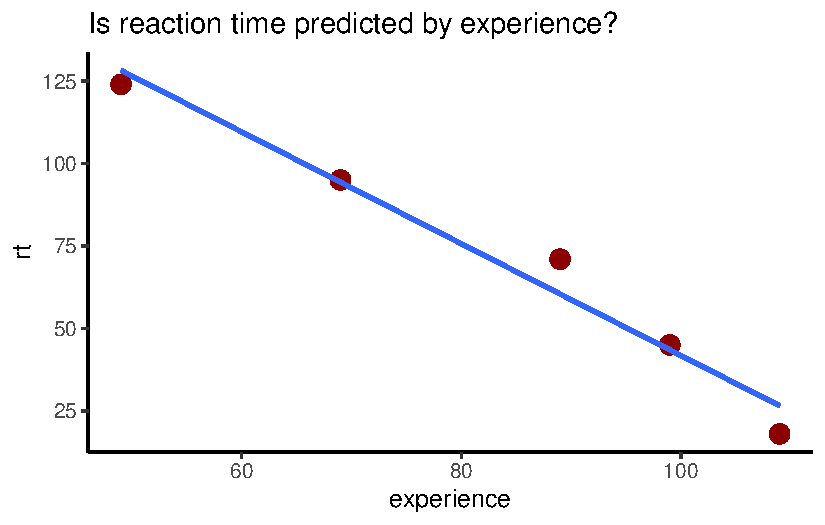
\includegraphics{model-fitting_files/figure-pdf/unnamed-chunk-2-1.pdf}

\subsection{Fitting Models in R}\label{fitting-models-in-r}

We will fit linear models using three common methods. During model
specification week, we already started fitting models with \texttt{lm()}
and \texttt{infer}. Today we will expand to include the \texttt{parsnip}
way.

\begin{enumerate}
\def\labelenumi{\arabic{enumi}.}
\item
  \textbf{\texttt{lm()}}: This is the most basic and widely used
  function for fitting linear models. It directly estimates model
  parameters based on the ordinary least-squares method, providing
  regression outputs such as coefficients, R-squared, etc.
\item
  \textbf{\texttt{infer} package}: This package focuses on statistical
  inference using tidyverse syntax. It emphasizes hypothesis testing,
  confidence intervals, and bootstrapping, making it ideal for
  inferential analysis.
\item
  \textbf{\texttt{parsnip} package}: Part of the \texttt{tidymodels}
  suite, \texttt{parsnip} provides a unified syntax for various modeling
  approaches (linear, logistic, random forest, etc.). It separates the
  model specification from the underlying engine, offering flexibility
  and consistency when working across multiple machine learning
  algorithms.
\end{enumerate}

Each method has its strengths: \texttt{lm()} for simplicity,
\texttt{infer} for inferential statistics, and \texttt{parsnip} for
robust model flexibility across different algorithms. To illustrate, we
can fit the data in the figure above all 3 ways.

\begin{Shaded}
\begin{Highlighting}[]
\CommentTok{\# with lm()}
\FunctionTok{lm}\NormalTok{(rt }\SpecialCharTok{\textasciitilde{}} \DecValTok{1} \SpecialCharTok{+}\NormalTok{ experience, }\AttributeTok{data =}\NormalTok{ data)}
\end{Highlighting}
\end{Shaded}

\begin{verbatim}

Call:
lm(formula = rt ~ 1 + experience, data = data)

Coefficients:
(Intercept)   experience  
    211.271       -1.695  
\end{verbatim}

\begin{Shaded}
\begin{Highlighting}[]
\CommentTok{\# with infer}
\NormalTok{data }\SpecialCharTok{\%\textgreater{}\%}
    \FunctionTok{specify}\NormalTok{(}\AttributeTok{formula =}\NormalTok{ rt }\SpecialCharTok{\textasciitilde{}} \DecValTok{1} \SpecialCharTok{+}\NormalTok{ experience) }\SpecialCharTok{\%\textgreater{}\%}
    \FunctionTok{fit}\NormalTok{()}
\end{Highlighting}
\end{Shaded}

\begin{verbatim}
# A tibble: 2 x 2
  term       estimate
  <chr>         <dbl>
1 intercept    211.  
2 experience    -1.69
\end{verbatim}

\begin{Shaded}
\begin{Highlighting}[]
\CommentTok{\# with parsnip }
\FunctionTok{linear\_reg}\NormalTok{() }\SpecialCharTok{\%\textgreater{}\%}
    \FunctionTok{set\_engine}\NormalTok{(}\StringTok{"lm"}\NormalTok{) }\SpecialCharTok{\%\textgreater{}\%}
    \FunctionTok{fit}\NormalTok{(rt }\SpecialCharTok{\textasciitilde{}} \DecValTok{1} \SpecialCharTok{+}\NormalTok{ experience, }\AttributeTok{data =}\NormalTok{ data)}
\end{Highlighting}
\end{Shaded}

\begin{verbatim}
parsnip model object


Call:
stats::lm(formula = rt ~ 1 + experience, data = data)

Coefficients:
(Intercept)   experience  
    211.271       -1.695  
\end{verbatim}

\subsection{Goodness-of-fit}\label{goodness-of-fit}

In order to find the best fitting free parameters, we first need to
quantify what it means to fit best. \textbf{Sum of squared error} (SSE)
is one common approach, in which we take the differences between the
data and the model fit -- 🥸 also called the ``error'' or ``residuals''
-- square those differences, and then take their sum.

\(SSE=\sum_{i=i}^{n} (d_{i} - m_{i})^2\)

\begin{itemize}
\tightlist
\item
  \(n\) is the number of data points
\item
  \(d_i\) is the \(i\)-th data point
\item
  \(m_i\) is the model fit for the \(i\)-th data point
\end{itemize}

Given this way of quantifying goodness-of-fit, our job is to figure out
the set of parameter values with the smallest possible sum of squared
error. But how do we do that? There are two common approaches:

\begin{enumerate}
\def\labelenumi{\arabic{enumi}.}
\tightlist
\item
  \textbf{Iterative Optimization} - works for both linear and nonlinear
  models
\item
  \textbf{Ordinary Least-Squares} - works for linear models only
\end{enumerate}

\subsection{Iterative Optimization}\label{iterative-optimization}

In \textbf{Iterative optimization}, we think of finding the best fitting
parameters as a \emph{search problem} in which we have a \emph{parameter
space} and a \emph{cost function} (or a ``loss'' function). To find the
best fitting parameter estimates, we search through the space to find
the point with the smallest possible cost function.

\begin{itemize}
\tightlist
\item
  We already have a cost function: sum of squared error

  \begin{itemize}
  \tightlist
  \item
    \(\sum_{i=i}^{n} (d_{i} - m_{i})^2\)
  \end{itemize}
\item
  We can visualize iterative optimization by plotting our cost function
  on the y-axis, and our possible paramter weights on the x-axis (and
  z-axis, and higher dimensions as the number of inputs goes up).
\item
  We call this visualizeation the \textbf{error surface}
\item
  If there is one parameter to estimate (one input to the model), the
  error surface will be a curvy line.
\end{itemize}

\begin{figure}

\begin{minipage}{0.50\linewidth}
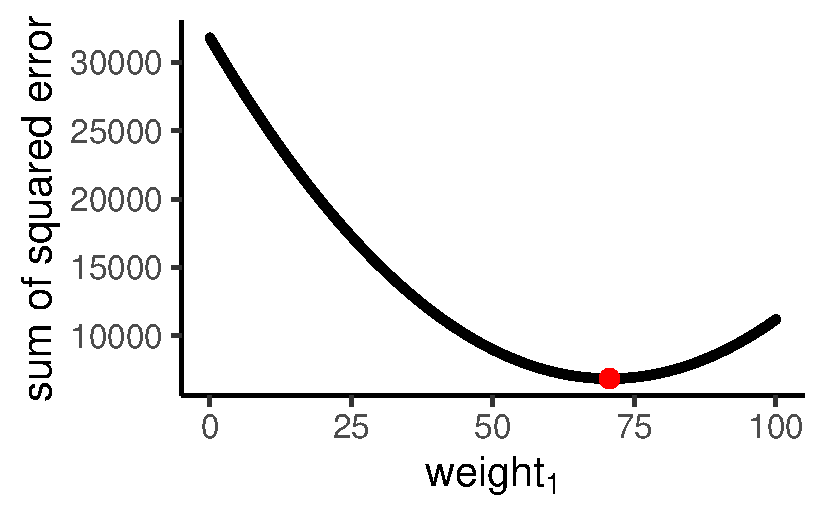
\includegraphics{model-fitting_files/figure-pdf/unnamed-chunk-5-1.pdf}\end{minipage}%

\end{figure}%

\begin{itemize}
\tightlist
\item
  If there are two parameters to estimate (two inputs to the model), the
  error surface will be a bumpy sheet.
\end{itemize}

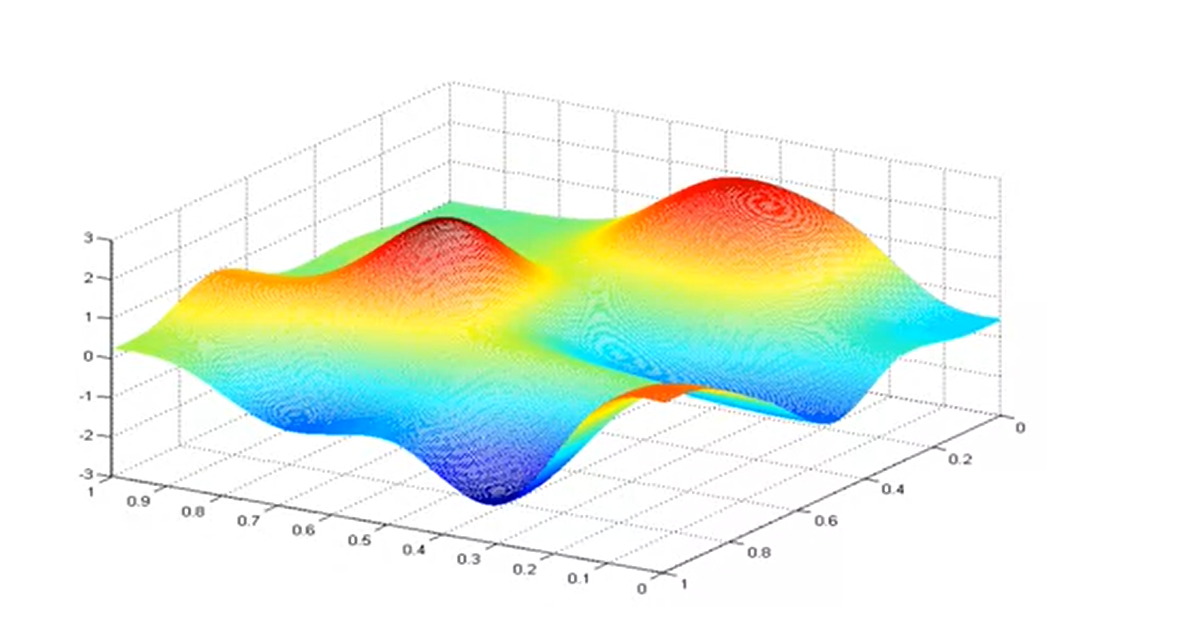
\includegraphics{../assests/images/error-surface.png}

To search through the parameter space via iterative optimization, we
could use any number of iterative optimization algorithms. Many of them
follow the same conceptual process (but differ in precise
implementation):

\begin{enumerate}
\def\labelenumi{\arabic{enumi}.}
\tightlist
\item
  Start at some point on the error surface (\emph{initial seed})
\item
  Look at the error surface in a small region around that point
\item
  Take a step in some direction that reduces the error
\item
  Repeat steps 2-4 until improvements are very small (less than some
  very small predefined number).
\end{enumerate}

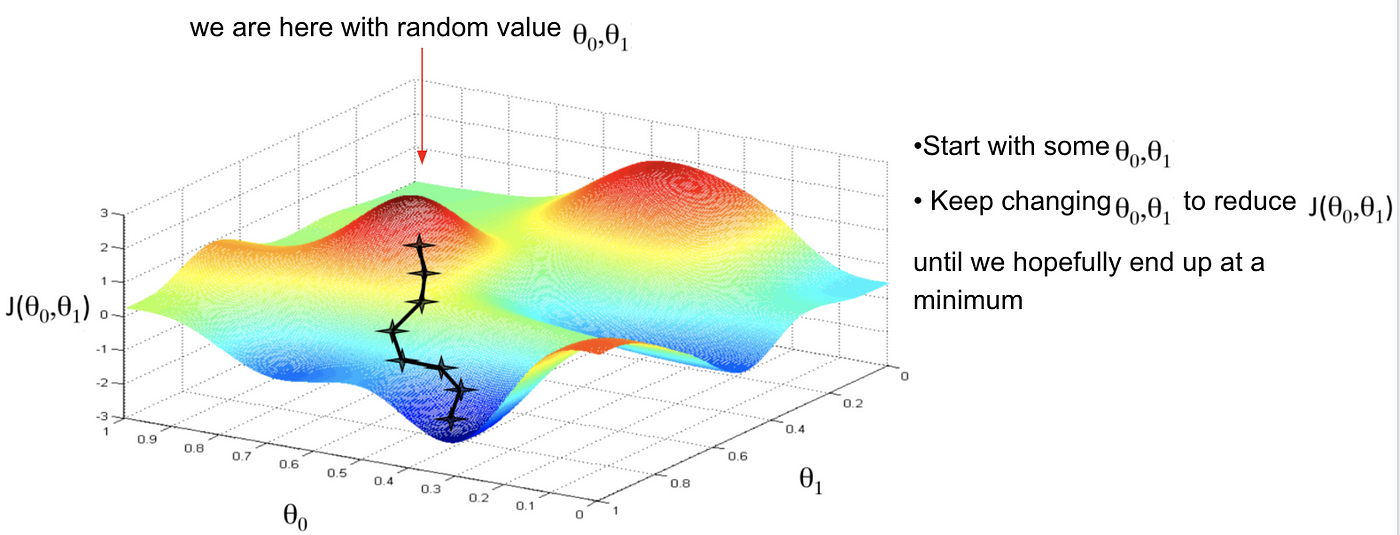
\includegraphics{../assests/images/gradient-descent.png}

If this feels too abstract, we can also understand iterative
optimization with a simple metaphor: suppose you were dropped from a
plane or helicopter at a random spot in hilly terrain and wanted to find
the lowest point. You could solve this with iterative optimization:

\begin{enumerate}
\def\labelenumi{\arabic{enumi}.}
\tightlist
\item
  Start at some point in the hilly terrain (\emph{inital seed})
\item
  Look around you to determine the direction in which the ground seems
  to be sloping downward the most.
\item
  Take a small step downhill in that direction.
\item
  Repeat these steps until you reach a spot where all directions around
  you either ascend or remain flat.
\end{enumerate}

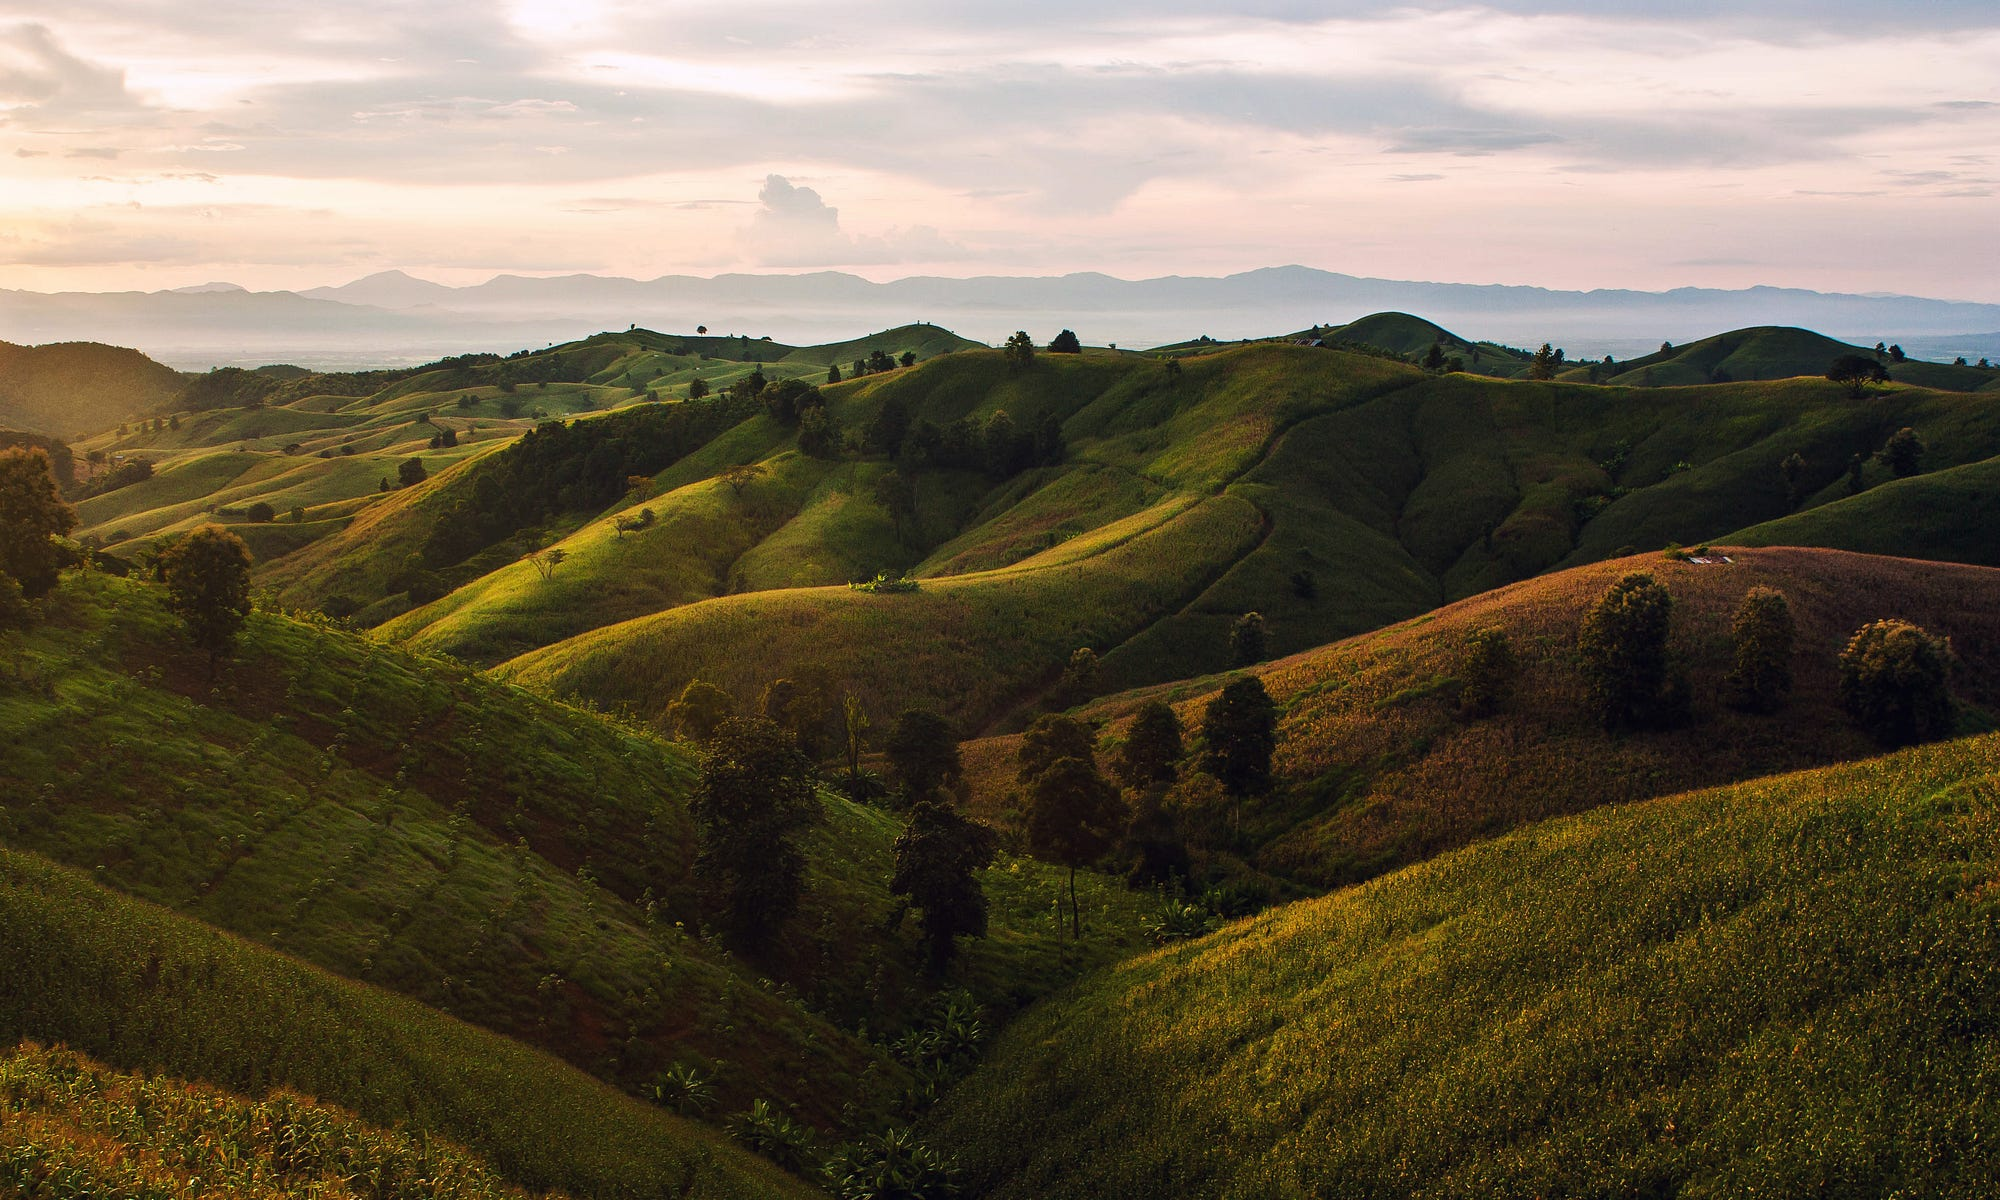
\includegraphics{../assests/images/grad-desc-intuition.jpeg}

\subsubsection{Gradient descent}\label{gradient-descent}

\textbf{Gradient descent} is one such iterative optimization algorithm.
We can implement gradient descent in R with the
\href{https://www.rdocumentation.org/packages/optimg/versions/0.1.2/topics/optimg}{\texttt{optimg}}
package to find the best fitting parameter estimates for our model.

\begin{enumerate}
\def\labelenumi{\arabic{enumi}.}
\tightlist
\item
  First we write our cost function --- our own function in R! --- which
  must take a \texttt{data} argument (our data set) and a \texttt{par}
  parameter (a vector of parameter estimates we want to test) to work
  with \texttt{optimg}.
\end{enumerate}

\begin{Shaded}
\begin{Highlighting}[]
\NormalTok{SSE }\OtherTok{\textless{}{-}} \ControlFlowTok{function}\NormalTok{(data, par) \{}
\NormalTok{    data }\SpecialCharTok{\%\textgreater{}\%}
        \FunctionTok{mutate}\NormalTok{(}\AttributeTok{prediction =}\NormalTok{ par[}\DecValTok{1}\NormalTok{] }\SpecialCharTok{+}\NormalTok{ par[}\DecValTok{2}\NormalTok{] }\SpecialCharTok{*}\NormalTok{ experience) }\SpecialCharTok{\%\textgreater{}\%}
        \FunctionTok{mutate}\NormalTok{(}\AttributeTok{error =}\NormalTok{ prediction }\SpecialCharTok{{-}}\NormalTok{ rt) }\SpecialCharTok{\%\textgreater{}\%}
        \FunctionTok{mutate}\NormalTok{(}\AttributeTok{squared\_error =}\NormalTok{ error}\SpecialCharTok{\^{}}\DecValTok{2}\NormalTok{) }\SpecialCharTok{\%\textgreater{}\%}
        \FunctionTok{with}\NormalTok{(}\FunctionTok{sum}\NormalTok{(squared\_error))}
\NormalTok{\}}
\end{Highlighting}
\end{Shaded}

\begin{enumerate}
\def\labelenumi{\arabic{enumi}.}
\setcounter{enumi}{1}
\tightlist
\item
  Then we pass our data, cost function, and initial seed paramters to
  the \texttt{optimg} function to perform gradient descent.
\end{enumerate}

\begin{Shaded}
\begin{Highlighting}[]
\FunctionTok{optimg}\NormalTok{(}
    \AttributeTok{data =}\NormalTok{ data,  }\CommentTok{\# our data}
    \AttributeTok{par =} \FunctionTok{c}\NormalTok{(}\DecValTok{0}\NormalTok{,}\DecValTok{0}\NormalTok{), }\CommentTok{\# our starting parameters}
    \AttributeTok{fn =}\NormalTok{ SSE,     }\CommentTok{\# our cost function (which receives data and par)}
    \AttributeTok{method =} \StringTok{"STGD"} \CommentTok{\# our iterative optimization algorithm }
\NormalTok{    )}
\end{Highlighting}
\end{Shaded}

\begin{verbatim}
$par
[1] 211.26155  -1.69473

$value
[1] 205.138

$counts
[1] 12

$convergence
[1] 0
\end{verbatim}

We can compare \texttt{optimg}'s estimates to that of \texttt{lm()} to
see that they are \emph{nearly} identical:

\begin{Shaded}
\begin{Highlighting}[]
\FunctionTok{lm}\NormalTok{(rt }\SpecialCharTok{\textasciitilde{}} \DecValTok{1} \SpecialCharTok{+}\NormalTok{ experience, }\AttributeTok{data =}\NormalTok{ data) }
\end{Highlighting}
\end{Shaded}

\begin{verbatim}

Call:
lm(formula = rt ~ 1 + experience, data = data)

Coefficients:
(Intercept)   experience  
    211.271       -1.695  
\end{verbatim}

\subsubsection{\texorpdfstring{Nearly identical to
\texttt{lm()}}{Nearly identical to lm()}}\label{nearly-identical-to-lm}

Note that solving for the best fitting free parameters via iterative
optimization gets us an \emph{approximate} value of the best fitting
free parameters. Based on how the algorithm is implemented, we might
decide to stop iterating too early (because we are close enough to the
point) or even step over minimum point if our step size is too big.

\subsubsection{Local minimum problem}\label{local-minimum-problem}

A potential problem with iterative optimization algorithms is the risk
of finding a \emph{local minimum}. That is, we find a location on the
error surface that is a minimum within some local range (so our
algorithm stops looking), but we are not at the absolute minimum (also
called the \emph{global minimum}).

\begin{itemize}
\tightlist
\item
  For all linear models, the error surface is shaped like a bowl, so
  there is \emph{no risk} of a local minimum. As long as an algorithm
  can adjust parameters to reduce errors, we will eventually be able to
  get to \emph{approximately} the optimal solution. We can see this
  clearly in the one or two parameter case (but it generalizes to higher
  dimensions as well).
\end{itemize}

Linear v. nonlinear model with one parameter:

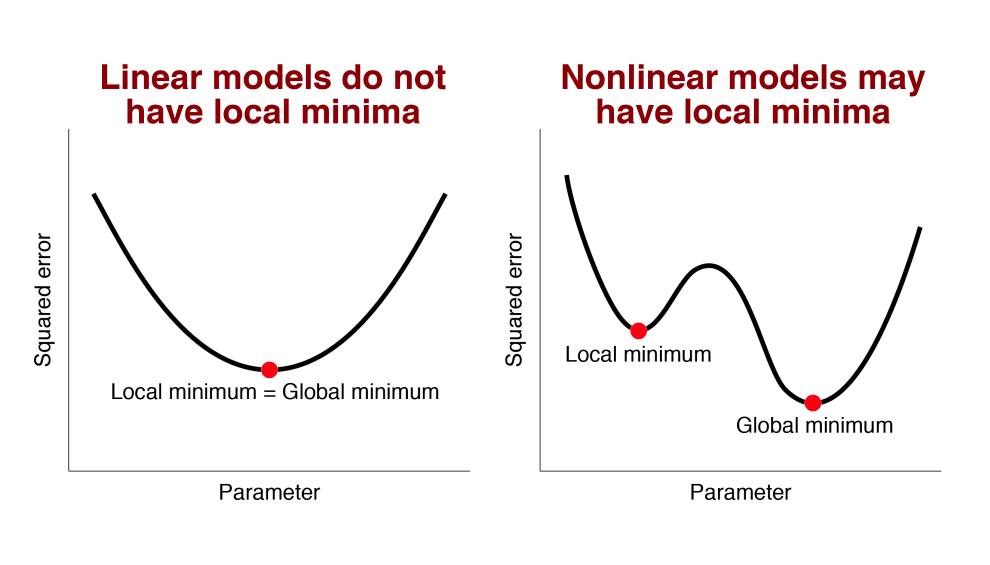
\includegraphics{../assests/images/local-v-global-min.png}

Linear model with two parameters:

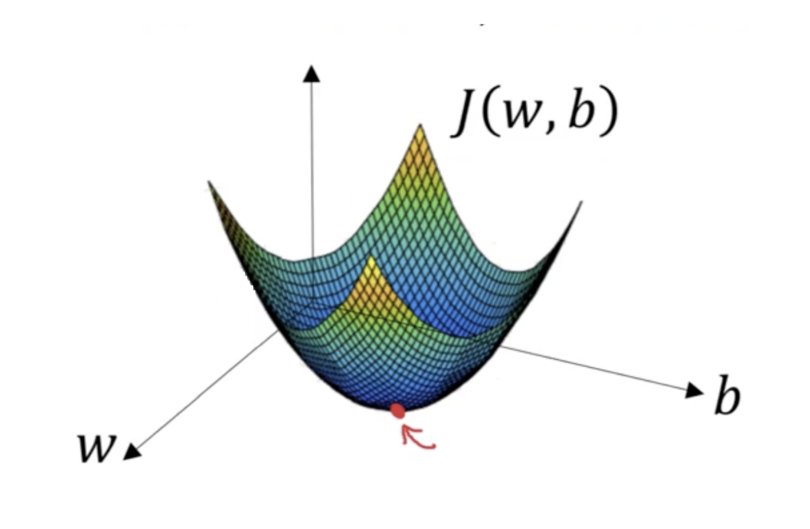
\includegraphics{../assests/images/grad-desct-linearmodel.png}

\subsection{Ordinary Least-Squares}\label{ordinary-least-squares}

Another way we can find the best fitting free parameters for linear (or
linearizable nonlinear) models is to use the Ordinary Least-Squares
(OLS) estimate.

\begin{itemize}
\tightlist
\item
  In OLS, the best-fitting free parameters are found by solving a system
  of equations (using matrix operations/linear algebra) which leads to a
  closed-form solution.\\
\item
  This means that OLS provides \emph{exact values} of the best-fitting
  parameters in one step (as long as a few necessary conditions are
  met).
\item
  We can contrast this with iterative optimization algorithms (like
  gradient descent) which gradually adjust the model parameters over
  multiple iterations to minimize the error, often requiring many steps
  to converge on \emph{approximate values} of the best-fitting
  parameters.
\end{itemize}

In OLS, the goal is to model the relationship between input variables
and the output variable (\(y\)) as a linear combination. We express this
very generally in our favorite equation, where the output (\(y\)) is a
weighted sum of inputs (\(x_i\)).

\begin{itemize}
\tightlist
\item
  \(y=\sum_{i=1}^{n}w_ix_i\)
\end{itemize}

Recall that this general expression has many 🥸 aliases. That is, the
\textbf{linear model equation} can be expressed in many ways, but
\emph{they are all this same thing}:

\begin{enumerate}
\def\labelenumi{\arabic{enumi}.}
\tightlist
\item
  in \textbf{high school algebra}: \(y=ax+b\).
\item
  in \textbf{machine learning}:
  \(y = w_0 + w_1x_1 + w_2x_2 + ... + w_nx_n\)
\item
  in \textbf{statistics}:
  \(y = β_0 + β_1x_1 + β_2x_2 + ... + β_nx_n + ε\)
\item
  in \textbf{matrix} notation: \(y = Xw + ε\)
\end{enumerate}

The matrix notation is what allows us to appreciate that we can solve
for the best fitting free parameters with linear algebra. Let's work
this out for our data set predicting
\texttt{rt\ \textasciitilde{}\ 1\ +\ experience}. We can express in
matrix notation:

\[
\begin{aligned}
    \mathbf{y} = \mathbf{X} \mathbf{w} + \mathbf{\epsilon}
\end{aligned}
\]

Where:

\begin{itemize}
\tightlist
\item
  \(\mathbf{y}\) is the output vector (\texttt{rt}).
\item
  \(\mathbf{X}\) is the input matrix (\texttt{experience} with an
  intercept).
\item
  \(\mathbf{w}\) is the weight vector (parameter estimates including the
  intercept).
\item
  \(\boldsymbol{\epsilon}\) is the vector of errors (residuals).
\end{itemize}

Because our data set is small, we can expand these to help you picture
this visually a little better:

\begin{enumerate}
\def\labelenumi{\arabic{enumi}.}
\tightlist
\item
  \textbf{Input Matrix} \(\mathbf{X}\) (intercept and
  \texttt{experience}):
\end{enumerate}

\[
\begin{aligned}
   \mathbf{X} = \begin{bmatrix}
   1 & 49 \\
   1 & 69 \\
   1 & 89 \\
   1 & 99 \\
   1 & 109
   \end{bmatrix}
\end{aligned}
\]

\begin{enumerate}
\def\labelenumi{\arabic{enumi}.}
\setcounter{enumi}{1}
\tightlist
\item
  \textbf{Output Vector}, \(\mathbf{y}\) (\texttt{rt}):
\end{enumerate}

\[
\begin{aligned}
   \mathbf{y} = \begin{bmatrix}
   124 \\
   95 \\
   71 \\
   45 \\
   18
   \end{bmatrix}
\end{aligned}
\]

\begin{enumerate}
\def\labelenumi{\arabic{enumi}.}
\setcounter{enumi}{2}
\tightlist
\item
  \textbf{Weight Vector}, \(\mathbf{w}\) (Unknown coefficients including
  intercept):
\end{enumerate}

\[
\begin{aligned}
   \mathbf{w} = \begin{bmatrix}
   w_1 \\  % Intercept
   w_2   % Weight for experience
   \end{bmatrix}
\end{aligned}
\]

Putting it all together, the linear model equation becomes, where there
is a vector of errors (residuals), \(\mathbf{\epsilon}\).

\[
\begin{aligned}
    \begin{bmatrix}
    124 \\
    95 \\
    71 \\
    45 \\
    18
    \end{bmatrix}
    =
    \begin{bmatrix}
    1 & 49 \\
    1 & 69 \\
    1 & 89 \\
    1 & 99 \\
    1 & 109
    \end{bmatrix}
    \begin{bmatrix}
    w_1 \\
    w_2
    \end{bmatrix}
    +
    \begin{bmatrix}
        \epsilon_1 \\
        \epsilon_2 \\
        \epsilon_3 \\
        \epsilon_4 \\
        \epsilon_5 \\
    \end{bmatrix}
\end{aligned}
\]

It turns out that we can solve for the weight vector directly via the
following equation:

\[
\begin{align}
\mathbf{w} = (\mathbf{X}^\top \mathbf{X})^{-1} \mathbf{X}^\top \mathbf{y}
\end{align}
\]

At this stage, we can take the mathematicians' word for it that this
provides an \emph{exact} solution to the best fitting parameter
estimates.

\begin{tcolorbox}[enhanced jigsaw, title=\textcolor{quarto-callout-tip-color}{\faLightbulb}\hspace{0.5em}{Box 1: Summary of OLS solution}, opacitybacktitle=0.6, toprule=.15mm, bottomtitle=1mm, colbacktitle=quarto-callout-tip-color!10!white, arc=.35mm, titlerule=0mm, toptitle=1mm, breakable, coltitle=black, bottomrule=.15mm, colback=white, colframe=quarto-callout-tip-color-frame, opacityback=0, leftrule=.75mm, left=2mm, rightrule=.15mm]

This is the end of the math we will uncover about the OLS in this
course. However, those of you who have taken linear algebra may
appreciate the following abridged summary of how we arrive at the closed
form solution by minimizing the sum of squared errors. (If you have not
taken linear alegebra, you can safely skip this box. It's not on the
exam!).

\[
\begin{align}
\mathbf{w} = (\mathbf{X}^\top \mathbf{X})^{-1} \mathbf{X}^\top \mathbf{y}
\end{align}
\]

To derive this we (in brief):

\begin{enumerate}
\def\labelenumi{\arabic{enumi}.}
\tightlist
\item
  \textbf{Set Up the Linear Model}: Start with the matrix equation
  \(\mathbf{y} = \mathbf{X} \mathbf{w} + \mathbf{\epsilon}\).
\item
  \textbf{Define Residuals}: Use
  \(\mathbf{\epsilon} = \mathbf{y} - \mathbf{X} \mathbf{w}\) to express
  the errors.
\item
  \textbf{Minimize SSE}: Expand and differentiate the sum of squared
  errors, setting the derivative to zero.
\item
  \textbf{Derive Normal Equation}: Arrive at the normal equation
  \(\mathbf{X}^\top \mathbf{X} \mathbf{w} = \mathbf{X}^\top \mathbf{y}\).
\item
  \textbf{Compute Weights}: Solve for \(\mathbf{w}\) using the
  closed-form solution.
\end{enumerate}

This process provides the \emph{exact} weights that best fit the linear
model to the data.

\end{tcolorbox}

We can demonstrate this with code:

\begin{Shaded}
\begin{Highlighting}[]
\NormalTok{ ols\_matrix\_way }\OtherTok{\textless{}{-}} \ControlFlowTok{function}\NormalTok{(X, Y)\{}
  \FunctionTok{solve}\NormalTok{(}\FunctionTok{t}\NormalTok{(X) }\SpecialCharTok{\%*\%}\NormalTok{ X) }\SpecialCharTok{\%*\%} \FunctionTok{t}\NormalTok{(X) }\SpecialCharTok{\%*\%}\NormalTok{ Y}
\NormalTok{ \}}
\end{Highlighting}
\end{Shaded}

We need to construct X and Y (must be matrices):

\begin{Shaded}
\begin{Highlighting}[]
\NormalTok{(response\_matrix }\OtherTok{\textless{}{-}}\NormalTok{ data }\SpecialCharTok{\%\textgreater{}\%} \FunctionTok{select}\NormalTok{(rt) }\SpecialCharTok{\%\textgreater{}\%} \FunctionTok{as.matrix}\NormalTok{())}
\NormalTok{(explanatory\_matrix }\OtherTok{\textless{}{-}}\NormalTok{ data }\SpecialCharTok{\%\textgreater{}\%} \FunctionTok{mutate}\NormalTok{(}\AttributeTok{int =} \DecValTok{1}\NormalTok{) }\SpecialCharTok{\%\textgreater{}\%} \FunctionTok{select}\NormalTok{(int, experience) }\SpecialCharTok{\%\textgreater{}\%} \FunctionTok{as.matrix}\NormalTok{())}
\end{Highlighting}
\end{Shaded}

\begin{figure}

\begin{minipage}{0.50\linewidth}

\begin{verbatim}
      rt
[1,] 124
[2,]  95
[3,]  71
[4,]  45
[5,]  18
\end{verbatim}

\end{minipage}%
%
\begin{minipage}{0.50\linewidth}

\begin{verbatim}
     int experience
[1,]   1         49
[2,]   1         69
[3,]   1         89
[4,]   1         99
[5,]   1        109
\end{verbatim}

\end{minipage}%

\end{figure}%

Then we can use our function to generate the OLS solution:

\begin{Shaded}
\begin{Highlighting}[]
\FunctionTok{ols\_matrix\_way}\NormalTok{(explanatory\_matrix, response\_matrix)}
\end{Highlighting}
\end{Shaded}

\begin{verbatim}
                   rt
int        211.270690
experience  -1.694828
\end{verbatim}

Which is \textbf{exactly the same} as that returned by \texttt{lm()}
(because lm is doing this!)

\begin{Shaded}
\begin{Highlighting}[]
\FunctionTok{lm}\NormalTok{(rt }\SpecialCharTok{\textasciitilde{}}\NormalTok{ experience, }\AttributeTok{data =}\NormalTok{ data)}
\end{Highlighting}
\end{Shaded}

\begin{verbatim}

Call:
lm(formula = rt ~ experience, data = data)

Coefficients:
(Intercept)   experience  
    211.271       -1.695  
\end{verbatim}

Importantly, if there are more regressors than data points, then there
is no OLS solution. The intuition for the underlying math is that if
there are more weights than data points, there are infinatly many
solutions, all of which acheive zero error. The linear algebra fans
among us might appreciate that the xtx component of our equation is
ill-defined in this case.

Here'a an example. Suppose we have the following dataset

\begin{Shaded}
\begin{Highlighting}[]
\NormalTok{data2 }\OtherTok{\textless{}{-}} \FunctionTok{tibble}\NormalTok{(}
    \AttributeTok{y =} \FunctionTok{c}\NormalTok{(}\DecValTok{2}\NormalTok{, }\DecValTok{5}\NormalTok{, }\DecValTok{7}\NormalTok{), }
    \AttributeTok{x =} \FunctionTok{c}\NormalTok{(}\DecValTok{1}\NormalTok{, }\DecValTok{2}\NormalTok{, }\DecValTok{3}\NormalTok{), }
    \AttributeTok{z =} \FunctionTok{c}\NormalTok{(}\DecValTok{2}\NormalTok{, }\DecValTok{4}\NormalTok{, }\DecValTok{6}\NormalTok{), }
    \AttributeTok{a =} \FunctionTok{c}\NormalTok{(}\DecValTok{6}\NormalTok{, }\DecValTok{7}\NormalTok{, }\DecValTok{8}\NormalTok{)}
\NormalTok{)}

\NormalTok{(model1 }\OtherTok{\textless{}{-}} \FunctionTok{lm}\NormalTok{(y }\SpecialCharTok{\textasciitilde{}} \DecValTok{1} \SpecialCharTok{+}\NormalTok{ x, }\AttributeTok{data =}\NormalTok{ data2))}
\end{Highlighting}
\end{Shaded}

\begin{verbatim}

Call:
lm(formula = y ~ 1 + x, data = data2)

Coefficients:
(Intercept)            x  
    -0.3333       2.5000  
\end{verbatim}

\begin{Shaded}
\begin{Highlighting}[]
\NormalTok{(model2 }\OtherTok{\textless{}{-}} \FunctionTok{lm}\NormalTok{(y }\SpecialCharTok{\textasciitilde{}} \DecValTok{1} \SpecialCharTok{+}\NormalTok{ x }\SpecialCharTok{+}\NormalTok{ z }\SpecialCharTok{+}\NormalTok{ a, }\AttributeTok{data =}\NormalTok{ data2))}
\end{Highlighting}
\end{Shaded}

\begin{verbatim}

Call:
lm(formula = y ~ 1 + x + z + a, data = data2)

Coefficients:
(Intercept)            x            z            a  
    -0.3333       2.5000           NA           NA  
\end{verbatim}

\texttt{lm()} is smart and fits the reduced model it \emph{can} fit. If
we try to solve this the matrix way via our homegrown function, we get
an error.




\end{document}
